\chapter{Thermal actuator driven with electrostatic currents}

\modinfo{Test}{ThermalActuator}
\modinfo{Directory}{ThermalActuator}
\modinfo{Solvers}{\Idx{StatCurrentSolve}, \Idx{HeatSolve}, 
	\Idx{StressSolve}}
\modinfo{Tools}{\Idx{ElmerGrid}, editor}
\modinfo{Dimensions}{3D, Steady-state}

\subsection*{Case definition}

The tutorial introduces a micro mechanical thermal actuator as shown
in Fig.~\ref{geom_thermal}. A static electric current is driven
through the actuator. The power loss due to the resistance of the
actuator is transformed into heat which in turn causes thermal
stresses into the structure. The electric current thus results in
deformation of the actuator. In industry, such an actuator might be
used to control the position of a micromechanical component.

\begin{figure}[h]
  \centerline{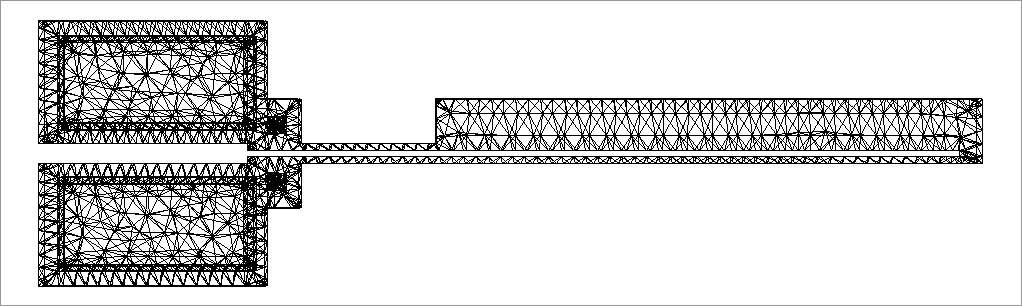
\includegraphics[width=0.8\textwidth]{geometry_wh}}
  \caption{The geometry of the actuator.} 
  \label{geom_thermal}
\end{figure}


\subsection*{Solution procedure}

The problem is solved by first iterating the electrostatic current
solver and heat equation until both are converged. The temperature
distribution is then used as a load for stress analysis solver which
calculates the actual deformation of the structure. The electric
conductivity of the actuator depends on the temperature and thus the
electrostatic - thermal problem is coupled in both directions.

The computational mesh for this particular tutorial is created by
using \Idx{Ansys} software. The details of the mesh are written into
files called \texttt{ExportMesh} by a certain Ansys macro and
converted to Elmer format by the ElmerGrid program. The command to use
is
\ttbegin
ElmerGrid 4 2 ExportMesh -order 1.0 0.1 0.001 -o thermal
\ttend 
The above command reads in the Ansys mesh files, arranges the mesh 
nodes in a reasonable way and saves the mesh in Elmer format in a
directory called \texttt{thermal}.

The geometry of the problem includes only one body and
material. Boundary conditions are defined on the actuator legs, which
are kept at constant electric potential, temperature and
position. Thus, only Dirichlet boundary conditions are used.

The header and simulation blocks of the solver input file are

\ttbegin
Header
  Mesh DB "." "thermal"
End

Simulation
  Coordinate System = Cartesian 3D
  Simulation Type = Steady State
  Steady State Max Iterations = 30
  Output Intervals = 1
  Output File = "actuator.result"
  Post File = "actuator.vtu"
End
\ttend

An initial condition for temperature is defined in order to ease the
convergence of the iterative solvers. Also, a body force for the
heat equation solver defining the Joule heating is needed. These
both have to be declared in the body section as follows:

\ttbegin
Body 1
  Equation = 1
  Material = 1
  Initial Condition = 1
  Body Force = 1
End
\ttend

The solution procedure requires the use of three solvers: Static
current solver, heat equation solver and the stress analysis
solver. The equation block below defines that these solvers are
used. 

\ttbegin
Equation 1
  Active Solvers(3) = Integer 1 2 3
  Calculate Joule Heating = True
End
\ttend

The solver blocks define the parameters of the respecting solvers. The
static current conduction problem is tackled by an iterative conjugate
gradient method (CG). For heat equation, a stabilized biconjugate
gradient method is used. The coupled problem of these two solvers is
difficult since the static current calculated heats the structure on
each step, and the rise of temperature makes the current conduction
more and more difficult. To overcome this problem, a relaxation factor
of 0.5 is defined for the heat equation solver.

\ttbegin
Solver 1
  Equation = Stat Current Solver
  Procedure = "StatCurrentSolve" "StatCurrentSolver"
  Variable = Potential
  Variable DOFs = 1
  Calculate Volume Current = True
  Calculate Electric Conductivity = True
  Linear System Solver = Iterative
  Linear System Iterative Method = CG
  Linear System Preconditioning = ILU3
  Linear System Max Iterations = 300
  Linear System Convergence Tolerance = 1.0e-8
  Nonlinear System Max Iterations = 1
  Nonlinear System Convergence Tolerance = 1.0-6
  Nonlinear System Newton After Iterations = 3
  Nonlinear System Newton After Tolerance = 1.0e-12
  Nonlinear System Relaxation Factor = 1.0
  Steady State Convergence Tolerance = 1.0e-6
End

Solver 2
   Equation = Heat Equation
   Variable = Temperature
   Variable DOFs = 1
   Linear System Solver = Iterative
   Linear System Iterative Method = BiCGStab
   Linear System Preconditioning = ILU1
   Linear System Max Iterations = 350
   Linear System Convergence Tolerance = 1.0e-9
   Nonlinear System Max Iterations = 1
   Nonlinear System Convergence Tolerance = 1.0e-07
   Nonlinear System Newton After Iterations = 3
   Nonlinear System Newton After Tolerance = 1.0e-12
   Nonlinear System Relaxation Factor = 0.5
   Steady State Convergence Tolerance = 1.0e-07
End
\ttend

For stress analysis, a direct solver is used instead of an iterative
solver. It is often difficult for the iterative solver to find a
solution for a structure that contains parts with varying stiffness
properties, which is obviously the case here (try the iterative solver
and see!). The stress analysis solver is called first only after the
coupled iteration of two previous solvers is complete. This is
possible since the deformation of the structure is so small that it
does not change the current density distribution. Defining stress
analysis this way saves computational time. It is possible to
iterate all the three solvers until convergence by commenting the
\texttt{Exec Solver} line.

\ttbegin
Solver 3
  Exec Solver = After All
  Equation = Stress Analysis
  Variable = Displacement
  Variable DOFs = 3
  Linear System Solver = Direct
  Linear System Direct Method = Banded
  Nonlinear System Max Iterations = 1
  Nonlinear System Convergence Tolerance = 1.0e-6
  Nonlinear System Newton After Iterations = 3
  Nonlinear System Newton After Tolerance = 1.0e-12
  Nonlinear System Relaxation Factor = 1.0
  Steady State Convergence Tolerance = 1.0e-6
End
\ttend

The material of the structure has a temperature dependent electric
conductivity. This, as well as other material parameters, is defined
in the material block. Note that a MEMS unit system is used.

\ttbegin
Material 1
  Electric Conductivity = Variable Temperature
      Real
        298.0   4.3478e10
        498.0   1.2043e10
        698.0   5.1781e9
        898.0   2.7582e9
        1098.0  1.6684e9
        1298.0  1.0981e9
        1683.0  1.0
        2000.0  1.0
      End

  Density = 2.3e-15
  Heat Conductivity = 32.0e6
  Youngs Modulus = 169.0e3
  Poisson Ratio = 0.22
  Heat Expansion Coefficient = 2.9e-6
  Reference Temperature = 298.0
End
\ttend

Finally, the initial condition, thermal heat load for stress analysis,
and the boundary conditions are defined.

\ttbegin
Initial Condition 1
   Temperature = 298.0
End

Body Force 1
  Heat Source = Equals Joule Heating
End

Boundary Condition 1
  Target Boundaries = 1
  Potential = 0
  Temperature = 298
  Displacement 1 = 0.0
  Displacement 2 = 0.0
  Displacement 3 = 0.0
End

Boundary Condition 2
  Target Boundaries = 2
  Potential = 7
  Temperature = 298
  Displacement 1 = 0.0
  Displacement 2 = 0.0
  Displacement 3 = 0.0
End
\ttend

\subsection*{Results}

The problem converges after 27 steady state iterations on the
tolerance limits defined above. The calculation takes about 180 cpu
seconds of which 40 cpus is spent in solving the stress analysis
equation. The calculations were performed on a Compaq Alpha Server
with a 1 GHz central processor.

\begin{figure}[tbhp]
  \centerline{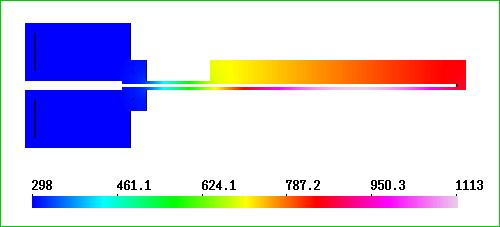
\includegraphics[width=0.8\textwidth]{temp_wh}}
  \caption{Temperature distribution.} 
  \label{temp_thermal}
\end{figure}
\begin{figure}[h]
  \centerline{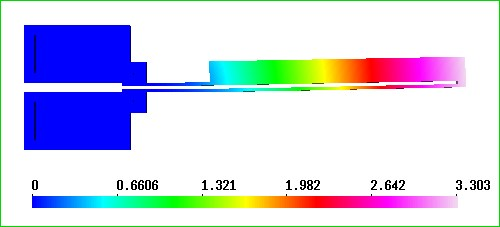
\includegraphics[width=0.8\textwidth]{displ_wh}}
  \caption{The displacement of the actuator.} 
  \label{displ_thermal}
\end{figure}

Result for temperature distribution and the displacement are shown in
Figs~\ref{temp_thermal} and~\ref{displ_thermal}. The temperature rises
unrealistically high in this example because all heat transfer
mechanisms out of the structure are neglected. Presumably at least
the heat radiation is of major importance in this case. For
displacement, the results show a movement of about 3.3 micrometers for
the actuator tip.

\vfill
\mbox{}
